\documentclass[tikz]{standalone}
\usepackage{tikz}
\usepackage[AutoFakeBold=true,AutoFakeSlant=true]{xeCJK}
\usepackage[zihao=-4,UTF8,heading=true]{ctex}
\usepackage[simplified]{pgf-umlcd}
\usetikzlibrary{positioning} %不加方向运算可能出错
\usetikzlibrary{arrows.meta} %箭头
\usetikzlibrary{calc}

\setCJKmainfont{微软雅黑}

\begin{document}
	\thispagestyle{empty}
    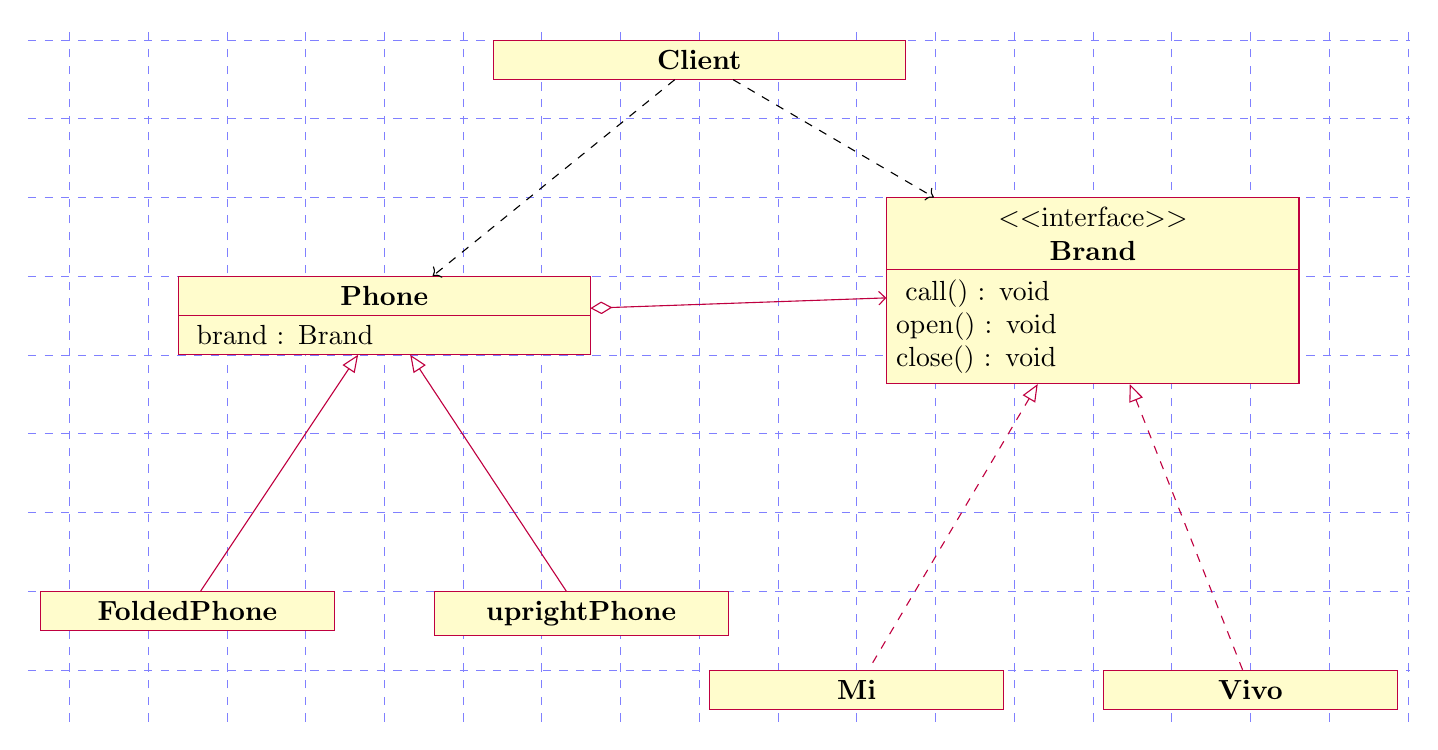
\begin{tikzpicture}[show background grid]
        \begin{class}[]{Client}{0, 10}
        
        \end{class}
        \begin{class}[]{Phone}{-4, 7}
            \attribute { brand : Brand }
        \end{class}
        \begin{interface}[]{Brand}{5, 8}
            \operation{ call() : void }
            \operation{ open() : void}
            \operation{ close() : void}
        \end{interface}
        \draw [dashed, ->] (Client) -- (Phone);
        \draw [dashed, ->] (Client) -- (Brand);
        \aggregation{Phone}{}{}{ Brand}
        
        \begin{class}[text width=3.5cm]{FoldedPhone}{-6.5, 3}
            \inherit{Phone}
        \end{class}
        \begin{class}[text width=3.5cm]{uprightPhone}{-1.5,3}
            \inherit{Phone}
        \end{class}
        \begin{class}[text width=3.5cm]{Mi}{2, 2}
            \implement{Brand}
        \end{class}
        \begin{class}[text width=3.5cm]{Vivo}{7, 2}
            \implement{Brand}
        \end{class}
        
        
    \end{tikzpicture}

\end{document}